\begin{tikzpicture}


\node (chain_setup) [wf-helpbox, text width=18em, anchor=west, font=\footnotesize] at (-8, 0) {
\texttt{\textbf{chain\_setup}(filename, cation, facets, ...):} \\ 
\textit{\begin{tabular}{l l}
& Set up a \texttt{cation} landscape for 2D wedges \\
& along a chain of \texttt{facets} for the molecule \\
& stored in \texttt{filename}.
\end{tabular}}
};

\node (sphere_setup) [wf-helpbox, text width=18em, anchor=east, font=\footnotesize] at (8, 0) {
\texttt{\textbf{sphere\_setup}(filename, cation, radius, ...):} \\ 
\textit{\begin{tabular}{l l}
& Set up a \texttt{cation} landscape for a sphere \\
& with a specified \texttt{radius} for the molecule \\
& stored in \texttt{filename}.
\end{tabular}}
};

\node (chain) [below=13.2em of chain_setup.west, anchor=west] {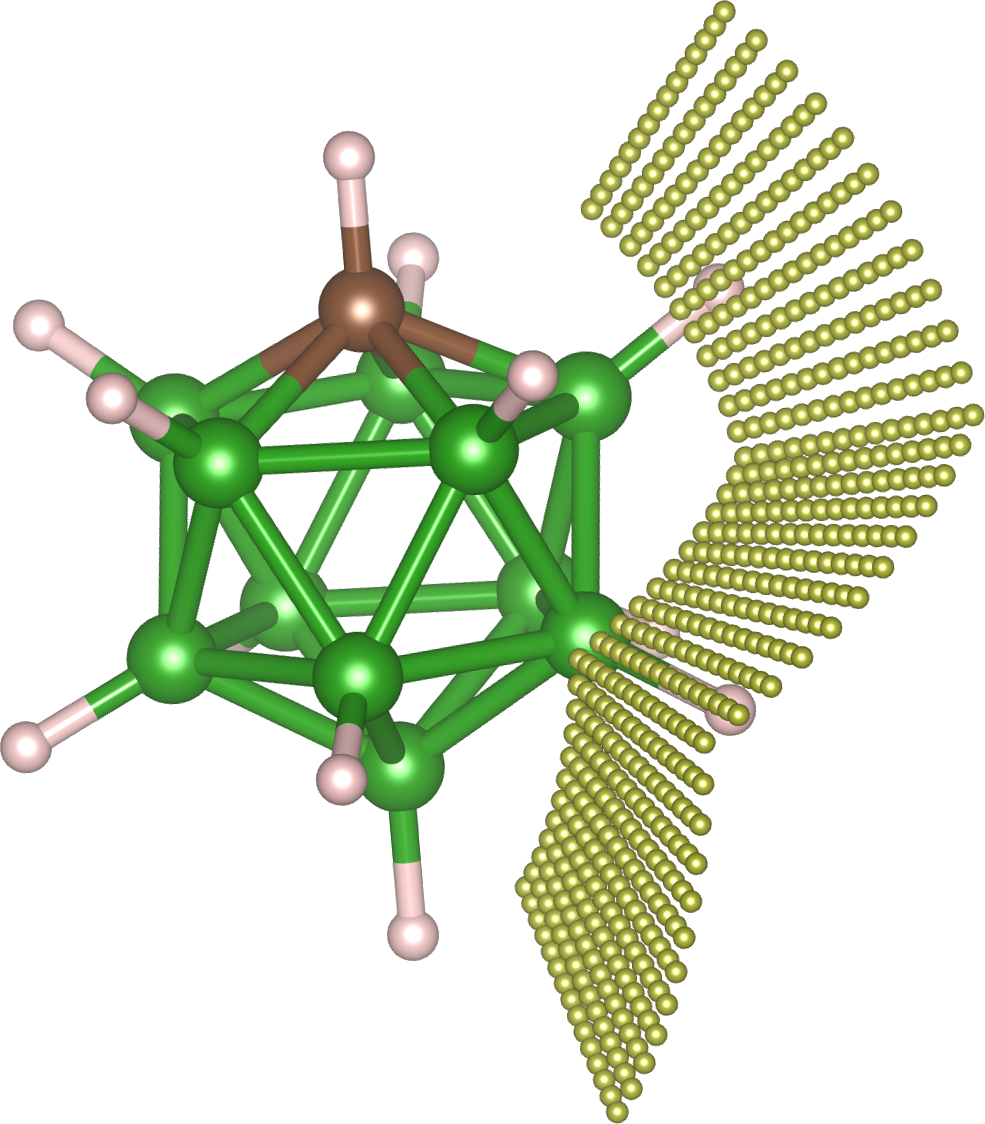
\includegraphics[width=140px]{\figurepath/automation/chain_landscape.png}};

\node (sphere) [below=13em of sphere_setup.east, anchor=east] {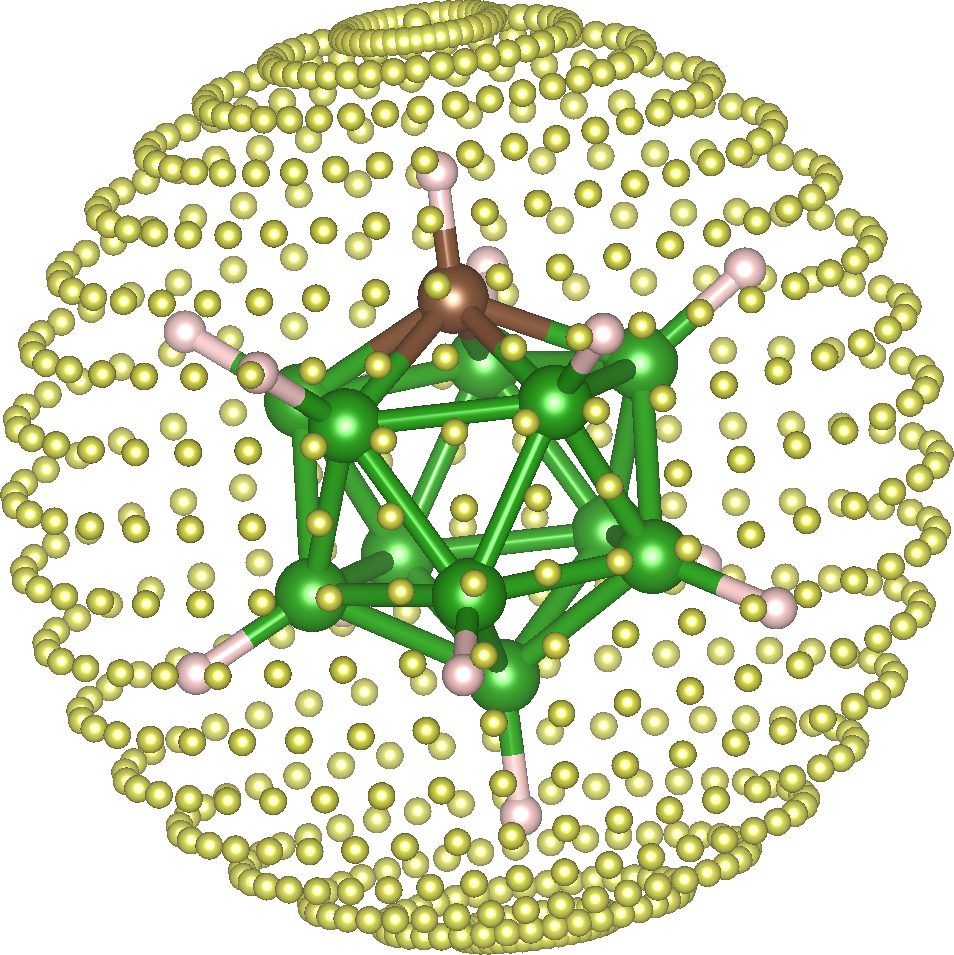
\includegraphics[width=150px]{\figurepath/automation/sphere_landscape.png}};

% Fireworks
\node (title_static1) [firework_name] at (0, -2) {StaticFW};
\node (static1_1) [firetask, below=0.2 em of title_static1] {\firetask{NWChemTask}};
\node (static1_2) [firetask, below=0.2 em of static1_1] {\firetask{ScriptTask}};

\begin{scope}[on background layer]
\node (frame_static1) [firework, fit={(title_static1) (static1_1) (static1_2)}] {}; 
\end{scope}

% Fireworks
\node (title_static2) [firework_name, below=1em of frame_static1] {StaticFW};
\node (static2_1) [firetask, below=0.2 em of title_static2] {\firetask{NWChemTask}};
\node (static2_2) [firetask, below=0.2 em of static2_1] {\firetask{ScriptTask}};

\begin{scope}[on background layer]
\node (frame_static2) [firework, fit={(title_static2) (static2_1) (static2_2)}] {}; 
\end{scope}

\node (dots) [below=1em of frame_static2] {...};

% Fireworks
\node (title_static3) [firework_name, below=1em of dots] {StaticFW};
\node (static3_1) [firetask, below=0.2 em of title_static3] {\firetask{NWChemTask}};
\node (static3_2) [firetask, below=0.2 em of static3_1] {\firetask{ScriptTask}};

\begin{scope}[on background layer]
\node (frame_static3) [firework, fit={(title_static3) (static3_1) (static3_2)}] {}; 
\end{scope}

\node (frame_wf) [draw, thick, rounded corners, fit={(frame_static1) (frame_static2) (frame_static3)}] {}; 

\draw [thick] ($(frame_wf.east) + (0, 6em)$) -- ($(frame_wf.east) + (5em, 6em)$);
\draw [thick] ($(frame_wf.west) + (0, 6em)$) -- ($(frame_wf.west) + (-5.5em, 6em)$);

\node (process_output) [wf-helpbox, text width=16em, below=27em of sphere_setup.east, anchor=east, font=\footnotesize] {
\textbf{\texttt{process\_output(output\_path):}} \\ 
\textit{\begin{tabular}{l l}
& Check the output in \textbf{\texttt{output\_path}}, \\ 
& load it in the \texttt{NwOutput} class\\
& and write it to a \texttt{.json} file. \\ 
\end{tabular}}
};

\node (helpbox1) [wf-helpbox, text width=14em, below=25em of chain_setup.west, anchor=west, font=\footnotesize] {
For each point in the energy landscape, a static calculation (\texttt{StaticFW}) is added to the workflow.
};

\coordinate (help1_bend) at ($(chain_setup.east) + (1em, 0em)$);
\draw [wf-helpline, ->, >=latex] (chain_setup.south) -- (chain.north -| chain_setup.south);
\draw [wf-helpline, ->, >=latex] (chain_setup.east) -- (help1_bend) -- (help1_bend |- frame_wf.north);
\coordinate (help2_bend) at ($(sphere_setup.west) + (-1em, 0em)$);
\draw [wf-helpline, ->, >=latex] (sphere_setup.south) -- (chain.north -| sphere_setup.south);
\draw [wf-helpline, ->, >=latex] (sphere_setup.west) -- (help2_bend) -- (help2_bend |- frame_wf.north);

\draw [wf-helpline] (static3_2.east) -- (static3_2.east -| process_output.north) -- (process_output.north);

\coordinate (help3_bend) at ($(helpbox1.north) + (6em, 5em)$);

\draw [wf-helpline] (helpbox1.north -| help3_bend) -- (help3_bend) -- (help3_bend -| frame_wf.west) ;

\end{tikzpicture}

